\documentclass[conference]{IEEEtran} % Clase IEEEtran para formato IEEE
\usepackage[utf8]{inputenc} % Codificación de caracteres
\usepackage[spanish]{babel} % Idioma español
\usepackage{amsmath, amssymb} % Paquetes para matemáticas
\usepackage{graphicx} % Paquete para incluir imágenes
\usepackage{cite} % Paquete para gestionar referencias
\usepackage{hyperref} % Paquete para hipervínculos
\usepackage{float} % Para forzar la posición de figuras


\title{Smart SSH Terminal} 
\author{
    \IEEEauthorblockN{Andres Felipe Gonzalez Garzon, Haider Andres Cañon Murcia}
    \IEEEauthorblockA{
        Bogotá, Colombia \\ 
        \texttt{andres-gonzalez16@upc.edu.co, Haider-canon@upc.edu.co} % [cite: 2]
    }
}

\begin{document}


\maketitle


\begin{abstract}
A lo largo de la historia de internet, los sistemas operativos han jugado 
un papel fundamental. En particular, los sistemas basados en Unix,
como Linux, constituyen la columna vertebral de la infraestructura que sostiene la red global.
Su administración se realiza principalmente a través de la terminal de línea de comandos. Este paper
propone una solución innovadora que integra un modelo de lenguaje grande (LLM) en un cliente SSH, 
facilitando la interacción y el aprendizaje en el entorno de la terminal.
\end{abstract}


\begin{IEEEkeywords}
SSH, Linux, LLM, Terminal Inteligente, cliente SSH, Administración de Sistemas, Asistente de IA, Unix/Linux
\end{IEEEkeywords}


\section{Introducción}
Desde los orígenes de la computación moderna, los sistemas operativos han 
sido el puente entre el ser humano y la máquina. Sin importar la época ni 
el fabricante, todos ellos han compartido un rasgo común: una interfaz de 
comandos textual que, si bien otorga un control preciso y profundo sobre el 
sistema, exige al usuario memorizar una sintaxis extensa, interpretar 
mensajes de error crípticos y construir mentalmente un modelo abstracto de 
cómo funciona el sistema \cite{shneiderman1982future}. Este escenario, que 
décadas atrás era exclusivo de especialistas, sigue siendo hoy el punto de 
entrada obligado para cualquier persona que aspire a comprender y gestionar 
sistemas operativos basados en Unix/Linux \cite{ritchie1974unix}. El 
resultado es documentado empíricamente: los mensajes de error de las 
herramientas de línea de comandos presentan una dificultad sustancial para 
los usuarios novatos \cite{becker2019compiler}; esta dificultad desencadena 
ciclos de frustración \cite{ossovski2024frustration} que, si se repiten sin 
retroalimentación efectiva, producen desenganche emocional progresivo de la 
tarea —patrón documentado en novatos de programación ante errores repetidos 
 \cite{bosch2017affective} y estructuralmente análogo al aprendizaje de 
entornos CLI, donde la misma ausencia de retroalimentación inmediata opera 
como factor de abandono. 

El auge reciente de los Modelos de Lenguaje Grande (LLMs) representa un 
punto de inflexión en este panorama. Por primera vez, es posible interactuar 
con sistemas complejos empleando lenguaje natural, recibir explicaciones 
contextuales al instante y obtener asistencia en la resolución de errores 
sin abandonar el entorno de trabajo \cite{brown2020language, chen2021evaluating}. 
Esta capacidad abre una oportunidad sin precedentes para transformar la 
forma en que los estudiantes y técnicos aprenden a operar un sistema 
operativo: no a través de la memorización pasiva, sino mediante la práctica 
guiada, contextual y progresiva \cite{denny2023conversing}. Sin embargo, en 
la práctica actual, la asistencia de IA permanece desacoplada del entorno 
donde ocurre el aprendizaje: el estudiante interrumpe su sesión de terminal, 
consulta un chatbot en el navegador y regresa al contexto de trabajo habiendo 
perdido tanto el flujo cognitivo como la trazabilidad del error. Para que el 
potencial pedagógico de los LLMs se materialice, la inteligencia artificial 
debe integrarse de forma nativa en el mismo espacio donde ocurre la 
práctica: la terminal remota. 

Precisamente de esa necesidad nace \textit{Smart SSH Terminal}: un entorno 
de trabajo integrado que fusiona en una sola interfaz el acceso remoto 
seguro vía SSH, la gestión de archivos por SFTP y un asistente de IA 
contextual que acompaña al usuario en tiempo real. La herramienta está 
dirigida tanto a estudiantes de ingeniería como a técnicos en formación que 
requieren un andamiaje inteligente para desarrollar competencias reales en 
el manejo de Linux en entornos de laboratorio remoto con recursos limitados. 
Estos requisitos de eficiencia de memoria, bajo consumo de CPU y seguridad 
en las comunicaciones motivaron la elección de Rust y el framework Tauri 
como base tecnológica \cite{klabnik2019rust}. 

Las soluciones existentes abordan estos problemas de forma parcial: los 
clientes SSH tradicionales carecen de componente pedagógico; las plataformas 
de aprendizaje interactivo de Linux no ofrecen acceso real a infraestructura 
remota; y los terminales modernos con IA como Warp presentan limitaciones 
funcionales sobre sesiones SSH remotas y no incorporan mecanismos de 
andamiaje progresivo \cite{warp2024ssh}. Ninguna herramienta integra 
simultáneamente acceso remoto autenticado, gestión de archivos y asistencia 
de IA pedagógica contextual en un único entorno. La Sección~II documenta 
este vacío en detalle. 

Las contribuciones principales de este trabajo son: (1) el diseño e 
implementación de \textit{Smart SSH Terminal}, un cliente SSH con asistente 
de IA integrado de forma nativa que transforma los errores de ejecución en 
retroalimentación pedagógica contextual; (2) una arquitectura eficiente en 
Rust y Tauri que satisface los requisitos de cómputo de servidores de 
laboratorio de bajo coste; y (3) una evaluación empírica del sistema sobre 
infraestructura real, con métricas de rendimiento (uso de CPU, memoria y 
latencia de respuesta). 

El resto del artículo se organiza así: la Sección~II revisa los trabajos 
relacionados; la Sección~III describe la arquitectura del sistema y sus 
subsistemas; la Sección~IV justifica las decisiones de implementación, en 
 particular la adopción de Rust; la Sección~V presenta la metodología de 
pruebas y los resultados en el laboratorio remoto; finalmente, las 
Secciones~VI y VII abordan el trabajo futuro y las conclusiones.

\section{Diseño Arquitectónico}

\subsection{Arquitectura General: Topología de Nodos y Subsistemas Distribuidos}

En un enfoque alineado con los patrones de diseño orientados a servicios (SOA) y despliegues telemáticos modernos, el sistema abandona el esquema tradicional de intermediarios centralizados. El diseño propone una topología distribuida donde el aplicativo principal reside encapsulado en la estación del estudiante como un \textbf{Cliente Inteligente (Smart Client)}, orquestando integraciones directamente frente a microservicios y hardware externo mediante una arquitectura orientada a eventos (EDA).

Como se ilustra en la Figura~\ref{fig:arquitectura_general}, la arquitectura propone una fuerte disociación entre la capa lógica de orquestación y el despliegue físico fáctico. El \textbf{Cliente Local} actúa como nodo orquestador hacia tres dominios externos: (1) el \textbf{Subsistema de Laboratorio Físico}, representado mediante un clúster IoT de baja latencia (ej. nodos Raspberry Pi) donde las actividades discurren sobre procesos nativos en Linux; (2) la \textbf{Nube de Inteligencia Artificial}, mediante el interfuncionamiento de inferencia en endpoints remotos LLM; y (3) el \textbf{Subsistema de Gestión Institucional}, compuesto por acoplamientos a plataformas LMS (Moodle) y directorios LDAP para salvaguardar la interoperabilidad de registro y federación de seguridad.

\begin{figure}[ht]
    \centering
    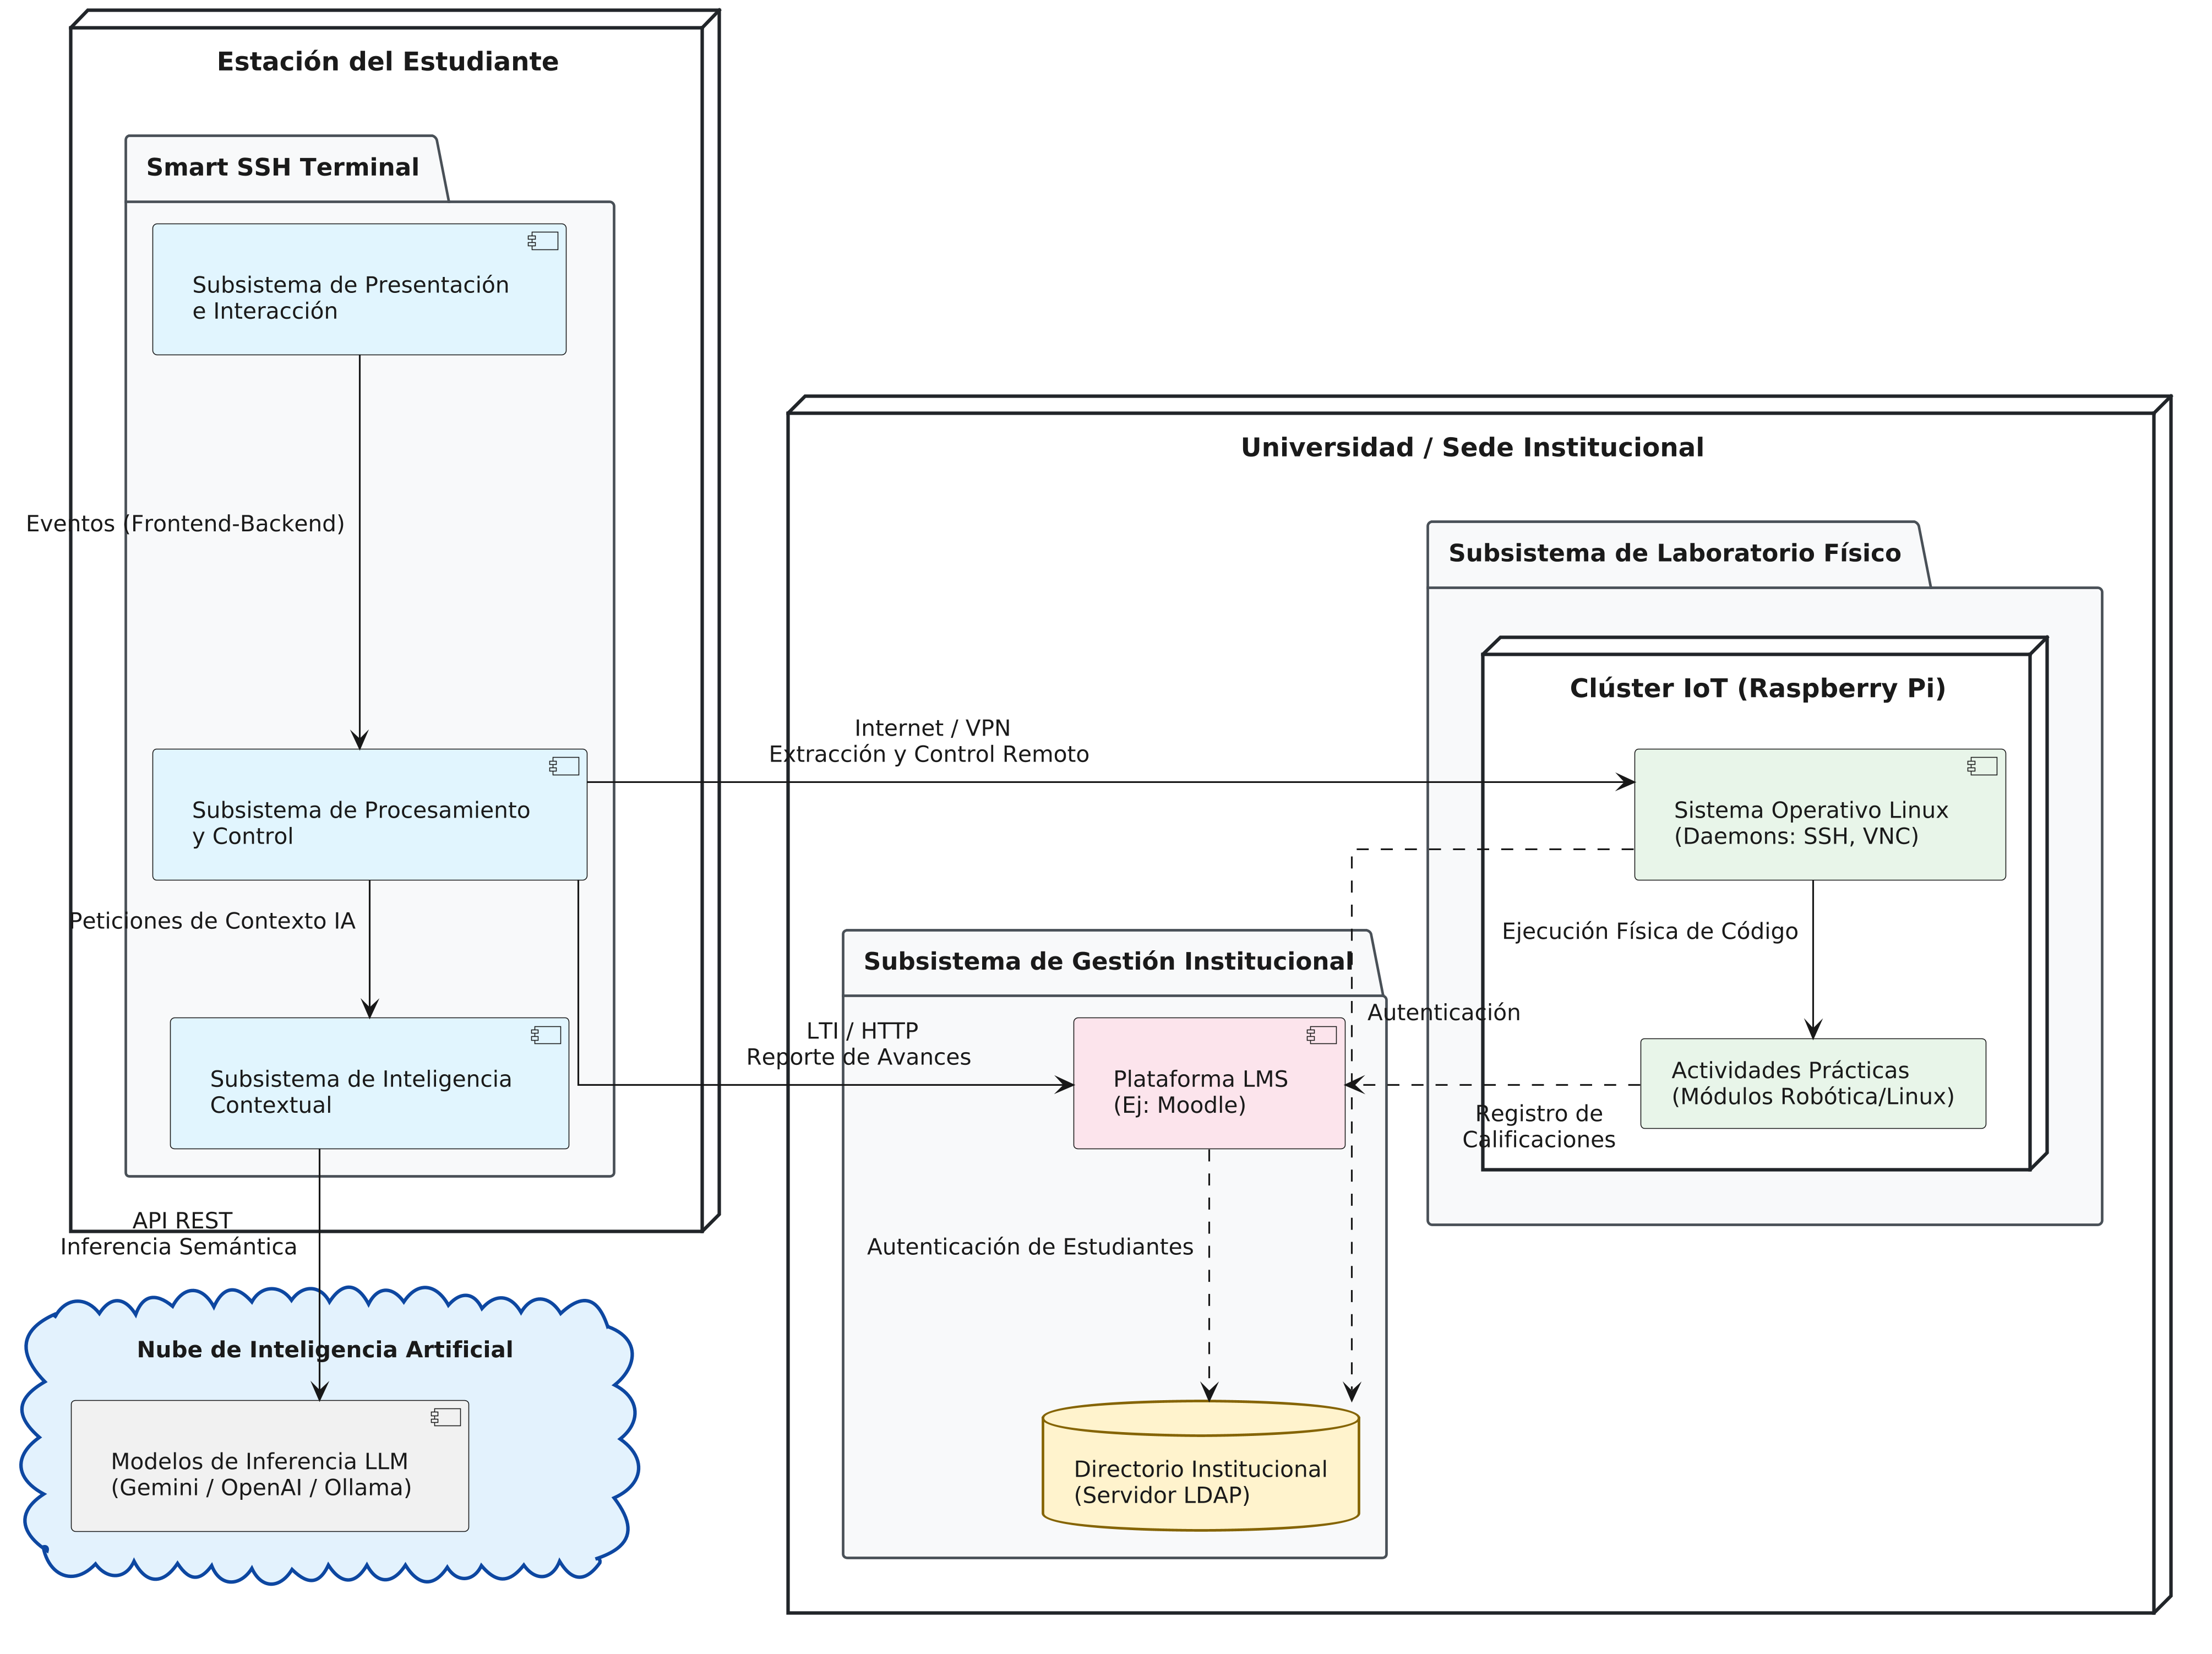
\includegraphics[width=\linewidth]{images/ar_ge_paper2.png}
    \caption{Topología general del sistema que demuestra la autonomía del cliente inteligente frente a integraciones modulares de sensórica IoT, software académico y servicios cognitivos en la nube.}
    \label{fig:arquitectura_general}
\end{figure}

A nivel interno, la lógica transaccional de la aplicación se subdivide en ecosistemas modulares desacoplados entre sí. A través de un bus de Comunicación entre Procesos (IPC), el sistema promueve los eventos asíncronamente, garantizando un aislamiento crítico: la interfaz visual simplemente actúa como un suscriptor de interfaz reactivo desprovisto de lógica directa de red. El subsistema frontal que asume la responsabilidad de la interfaz es el \textbf{Subsistema de Presentación e Interacción}, que engloba el emulador de terminal, la gestión gráfica de archivos y el chat conversacional.

\subsection{Subsistema de Procesamiento y Control (Core)}

El motor principal (Core), construido como un demonio local orientado a concurrencia y seguridad de memoria asíncrona, funge como el cerebro orquestador de las comunicaciones de bajo nivel (ver Figura~\ref{fig:subsistema_nucleo}):
\begin{itemize}
    \item \textbf{Canal de Transporte Cifrado en Capa Lógica}: Implementación estructural y multiplexada del protocolo Secure Shell (SSH), facilitando un acoplamiento directo entre flujos criptográficos del cliente emulador y los daemons expuestos por los nodos de la topología IoT remota.
    \item \textbf{Agente de Trazabilidad I/O}: Actuando en sintonía bajo el paradigma de Event-Driven Architecture, un demonio subyacente inspecciona la entrada/salida (I/O) ejecutada a nivel de socket; proveyendo una fragmentación estructurada en una bitácora temporal inmutable para ser sujeta a análisis.
\end{itemize}

\begin{figure}[ht]
    \centering
    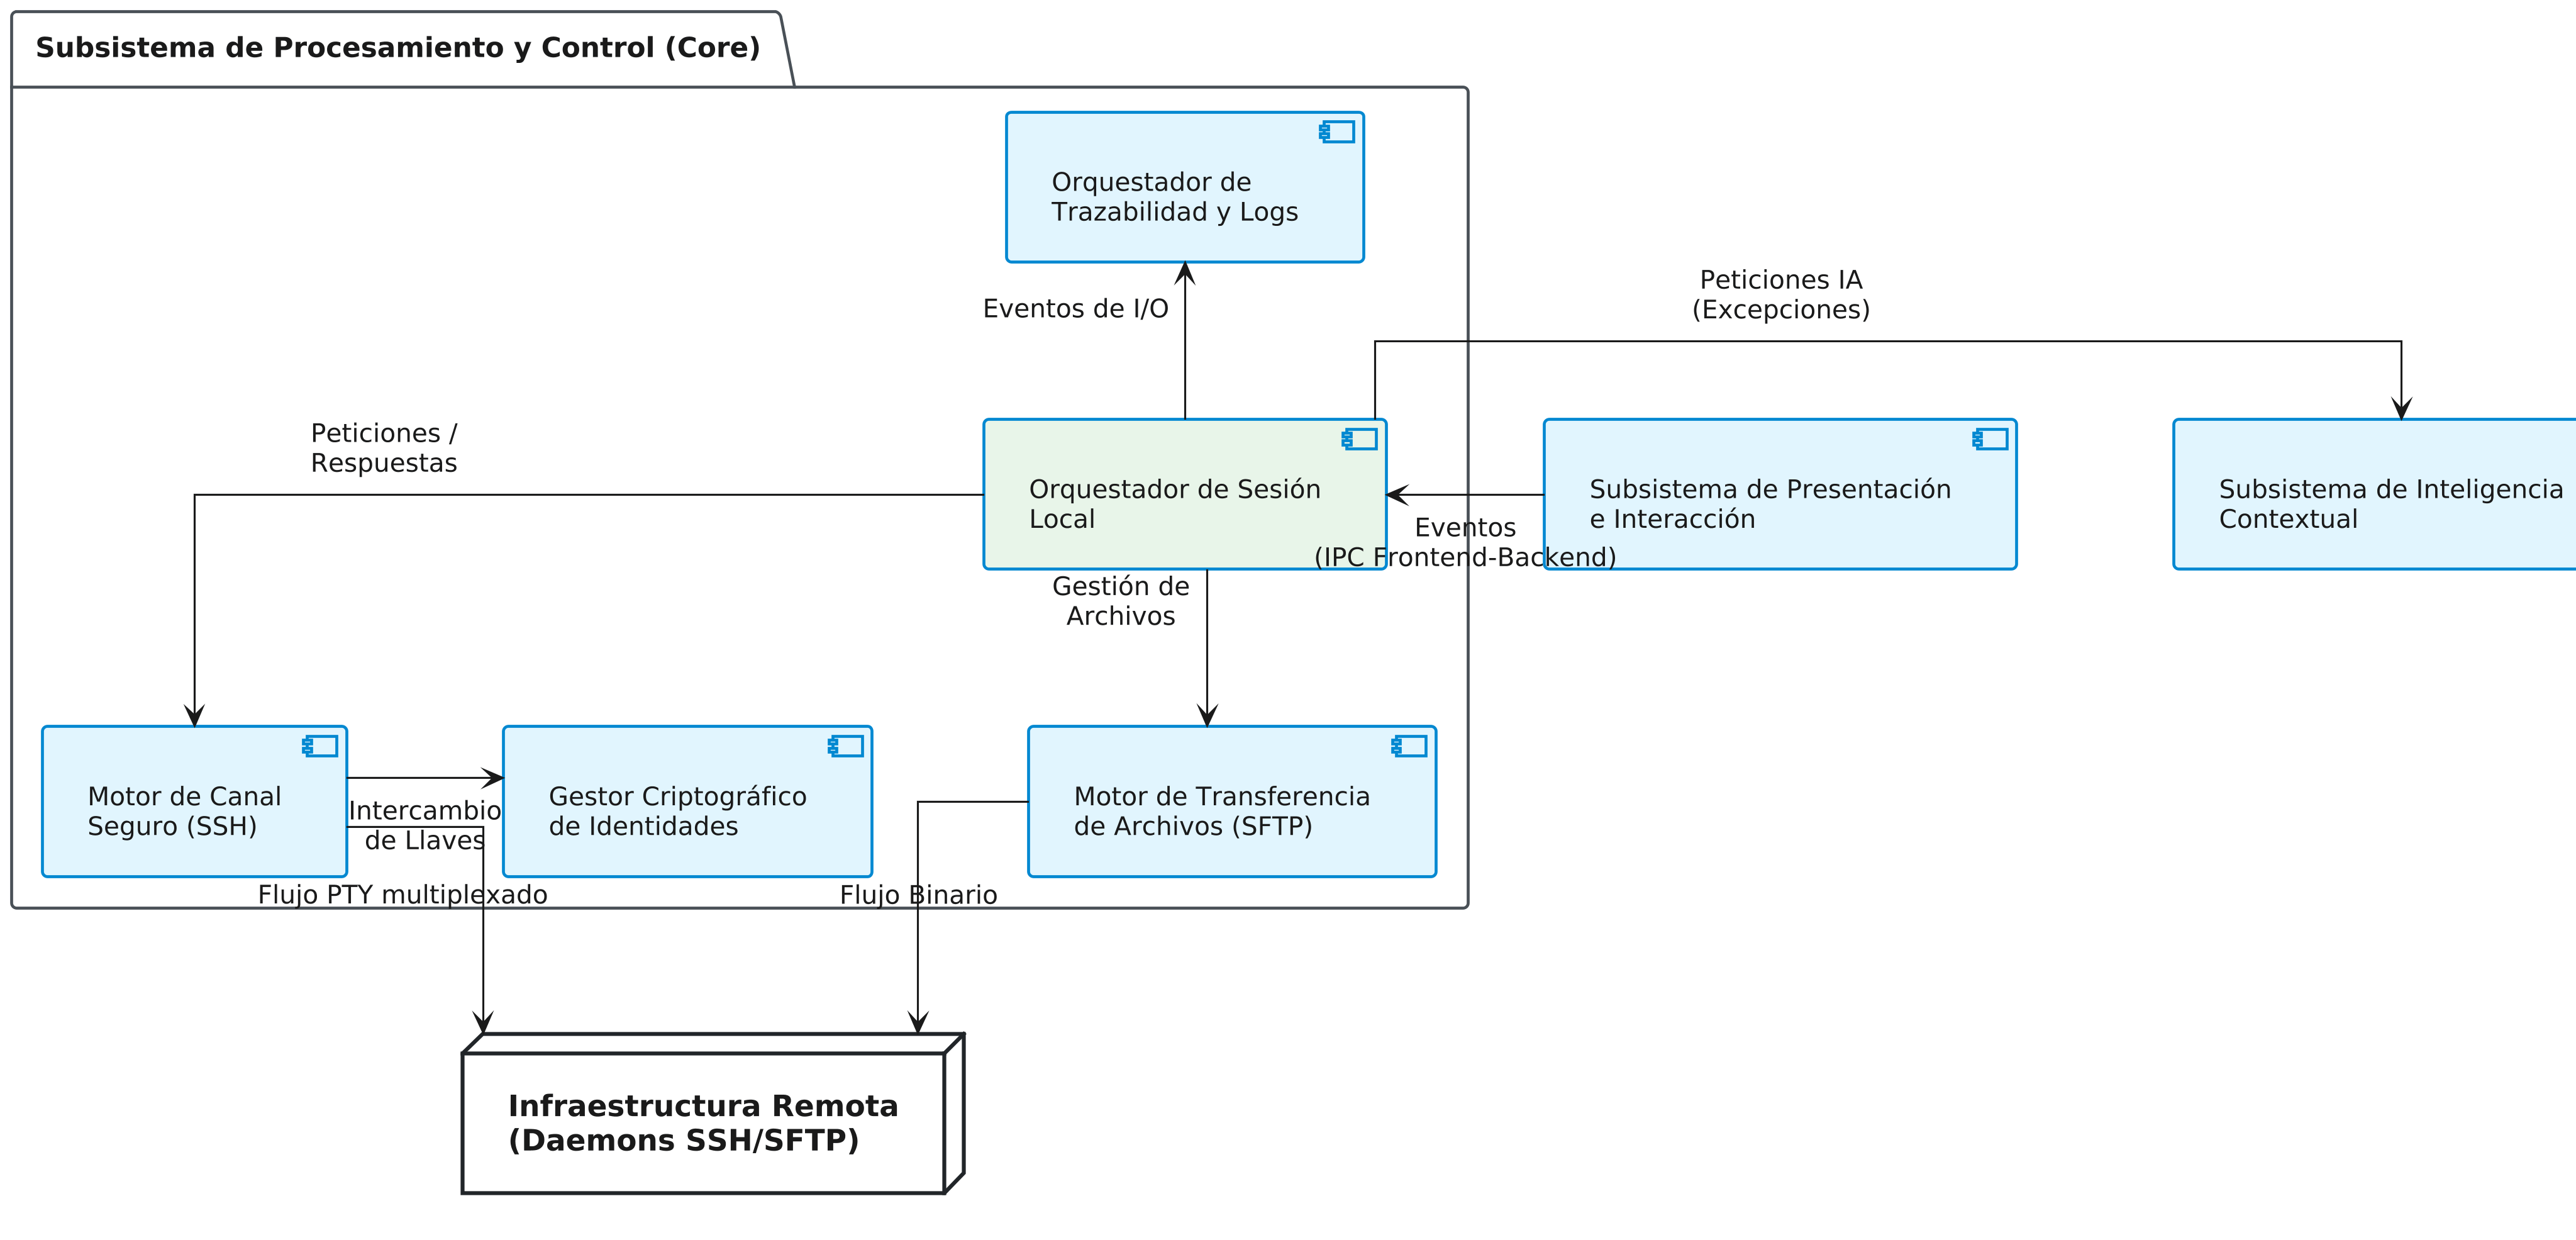
\includegraphics[width=\linewidth]{images/subsistema_nucleo.png}
    \caption{Diseño del Subsistema Transaccional para la orquestación distribuida de canales SSH/SFTP e interceptación de eventos de sesión local.}
    \label{fig:subsistema_nucleo}
\end{figure}

\subsection{Subsistema de Inteligencia Contextual (Agente)}

Con el imperativo de reducir la ambigüedad computacional y posibilitar andamiajes pedagógicos predecibles, la topología destina una capa lógica final a procesar la semántica transaccional (Figura~\ref{fig:subsistema_agente}). Lejos del paradigma conversacional estándar, este subsistema ejecuta inferencias sobre manifiestos técnicos recolectados automáticamente:

\begin{itemize}
    \item \textbf{Descubrimiento Sensible al Contexto (Context Protocol)}: Dotación técnica de middleware que, antes de escalar solicitudes a la nube LLM remota, procesa sistemáticamente los *logs* de terminal y descriptores de red locales. Esto enhebra eventos lógicos para entregarle al servicio de razonamiento una radiografía fáctica del estado remoto del laboratorio y los posibles atascos sintácticos.
    \item \textbf{Motor Ontológico de Prácticas Guiadas}: Autómata evaluador local que contrasta asíncronamente las interacciones extraídas en los nodos IoT frente a ontologías descriptivas (fases y misiones) definidas en un contexto formativo, mitigando derivas temáticas al accionar la inteligencia cognitiva contextual.
\end{itemize}

\begin{figure}[ht]
    \centering
    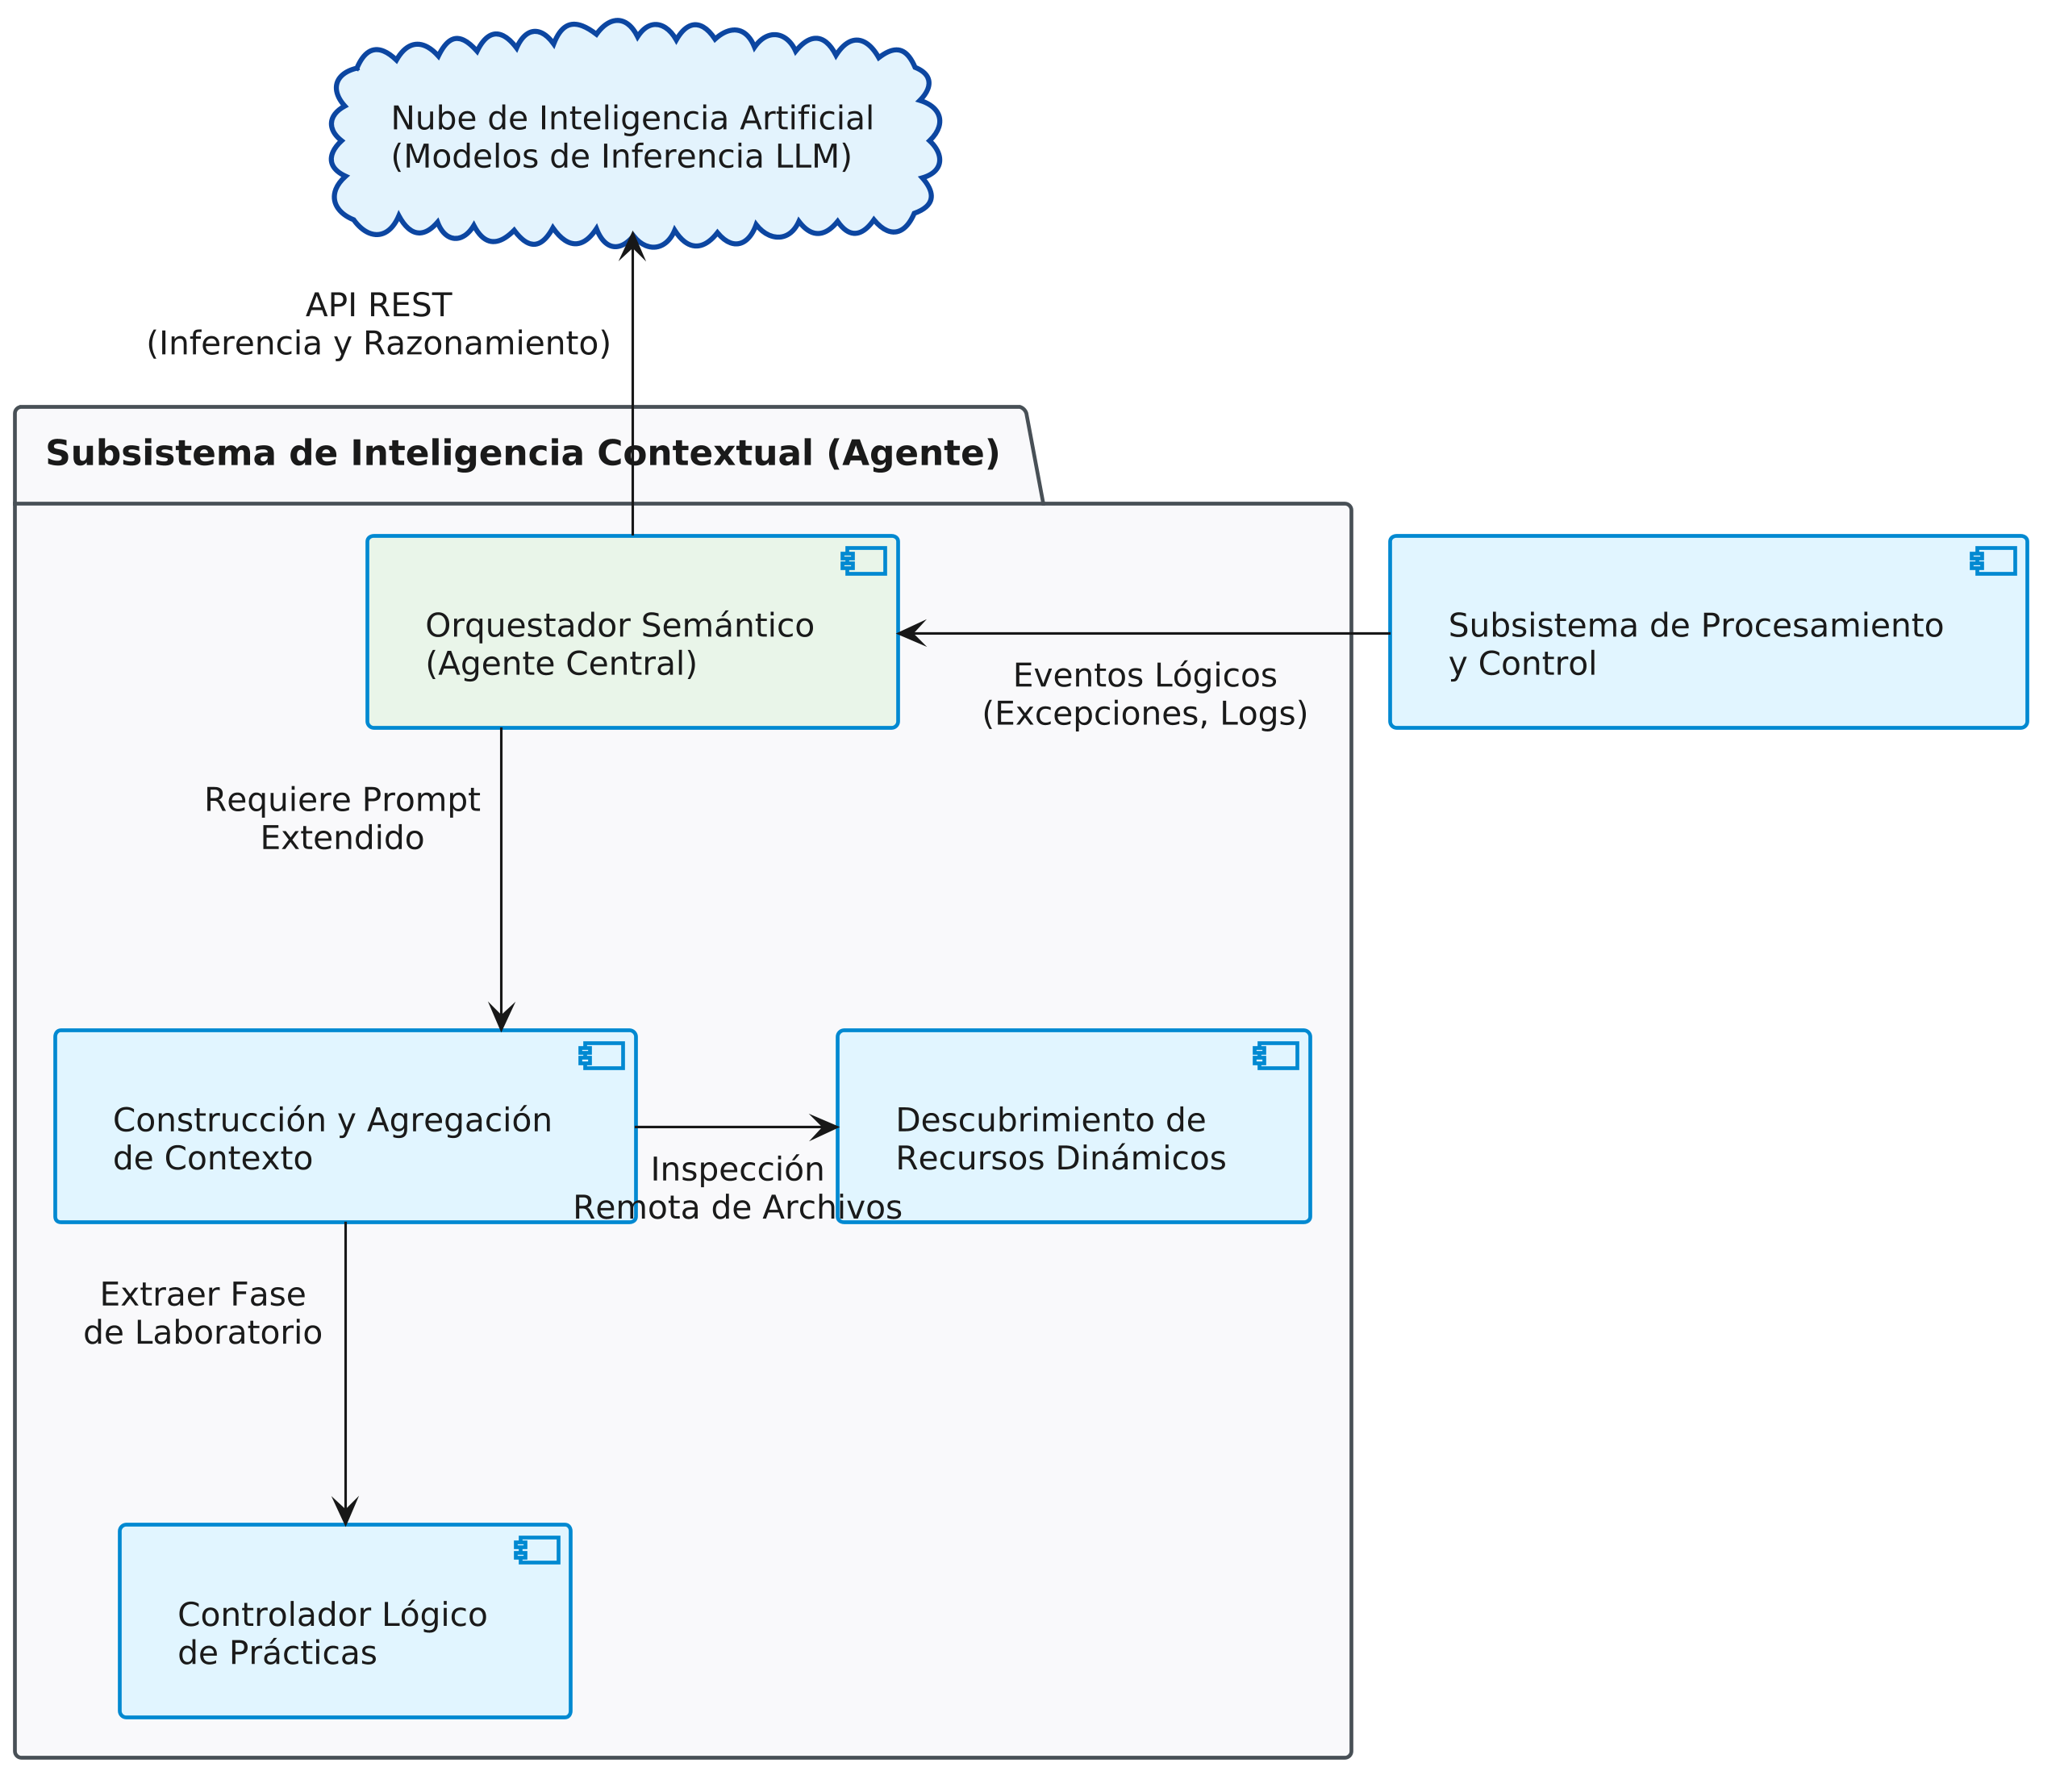
\includegraphics[width=\linewidth]{images/subsistema_agente.png}
    \caption{Estructura de la Capa Semántica enfocada en el protocolo de contexto pragmático y orquestación a endpoints proveedores de Modelos de Lenguaje.}
    \label{fig:subsistema_agente}
\end{figure}

\subsection{Integración Arquitectónica y Beneficios Subyacentes}

La topología expuesta erradica la fragmentación típica encontrada en clientes remotos \cite{mobaxterm_misc}. La consolidación de canales (como conexiones SSH reusadas y WebSockets noVNC para escritorios virtuales) fusionados con un servicio \textit{endpoint} inteligente reduce de forma abismal la latencia cognitiva de transición. El estudiante experimenta un \textit{sandbox} único en donde errores operacionales son inmediatamente atrapados y digeridos semánticamente para proponer un apoyo educativo ininterrumpido.

\subsection{Subsistema de Gestión Institucional (Gobernanza LMS)}

De importancia crítica, y ontológicamente superior dentro del ciclo de vida de la aplicación tecnológica, se proyecta la integración bilateral con las Plataformas de Gestión de Aprendizaje Institucionales (LMS), tales como Moodle. Aunque la infraestructura de telemetría inmersiva y la inteligencia artificial habilitan laboratorios aislados de alto impacto, el verdadero valor fundacional reside en la Gobernanza Pedagógica otorgada al cuerpo docente.

A nivel arquitectónico, el agente local orquesta reportes perimetrales mediante el estándar \textit{Learning Tools Interoperability} (LTI) o API REST (figurativamente encapsulados en el Subsistema de Gestión Institucional). Esto traslada la carga de evaluación del evaluador humano al motor automatizado local, proveyendo:
\begin{itemize}
    \item \textbf{Despliegue y Autoría de Prácticas}: Permite a los profesores diseñar o cargar manifiestos de laboratorios (con fases, objetivos técnicos, distribuciones de servidor y comandos permitidos) directamente en el LMS, los cuales son interpretados topológicamente por el cliente Smart SSH.
    \item \textbf{Monitorización Telemétrica en Tiempo Real}: Los docentes adquieren una ventana estructurada para auditar en vivo las métricas de éxito (comandos acertados vs comandos asistidos por la IA) por cada clúster.
    \item \textbf{Consolidación de Calificaciones (Gradebook Sync)}: Una vez el autómata lógico reconoce el cumplimiento de una práctica (basado en la verificación de binarios y salidas de consola alteradas temporalmente), sincroniza de forma opaca y cifrada la evaluación obtenida directamente al libro de notas (Gradebook) de Moodle.
\end{itemize}

Esta interconexión eleva al cliente desde un simple emulador de administración de redes hacia una poderosa solución llave en mano de \textit{Learning Analytics}, indispensable en entornos formales universitarios.

\section{Implementación}
\subsection{Evolución del desarrollo}
El desarrollo de esta herramienta comenzó inicialmente utilizando Tkinter, debido a que representaba la vía más rápida para prototipar una interfaz gráfica básica. Sin embargo, durante esta etapa se identificaron problemas críticos relacionados con el refresco de pantalla y la fluidez necesaria para un emulador de terminal en tiempo real.

\subsection{Justificación de Rust}
Ante las limitaciones de rendimiento encontradas, se decidió realizar un salto tecnológico hacia Rust \cite{klabnik2019rust}. Este lenguaje fue elegido por su enfoque en la seguridad de memoria \cite{jung2017rustbelt}, su alto rendimiento comparable al de C/C++ \cite{levy2017rust}, y su ecosistema moderno que facilita la creación de aplicaciones de escritorio seguras. Rust permite una gestión eficiente de hilos y una respuesta inmediata en la interfaz de usuario.

\subsection{Integración de servicios}
La aplicación actual ya incorpora servicios equivalentes a los ofrecidos por herramientas tradicionales como WinSCP \cite{mobaxterm_misc}, permitiendo la gestión gráfica de archivos mediante el protocolo SFTP de forma integrada con la terminal.

\subsection{La Novedad}
La principal innovación radica en haber logrado una interfaz limpia y amigable que no solo emula una terminal, sino que es capaz de realizar un seguimiento inteligente a las acciones del usuario, ofreciendo asistencia contextual proactiva sin sobrecargar la experiencia de uso.

\section{Escenario de Pruebas}
\label{sec:pruebas}
\subsection{Metodología}
Para validar la herramienta, se llevó a cabo una metodología de pruebas con un grupo de 10 personas con distintos niveles de experiencia en Linux. El objetivo fue evaluar la facilidad de uso y la efectividad de la asistencia por IA.

\subsection{Métricas y gráficas}
Los resultados mostraron tiempos de uso promedio de 20 minutos de interacción continua, durante los cuales los usuarios lograron generar comandos complejos y realizar tareas de administración que normalmente requerirían consultas externas a la documentación.

\subsection{Laboratorio remoto}
La interfaz permite acoplarse a un escenario de laboratorio remoto \cite{garcia2010web}, como el uso de una Raspberry Pi \cite{de2011virlab}. Esto permite a los usuarios desarrollar prácticas reales mientras monitorean el entorno físico. A continuación se presentan fotografías de evidencia del funcionamiento en este entorno.

\begin{figure}[H]
    \centering
    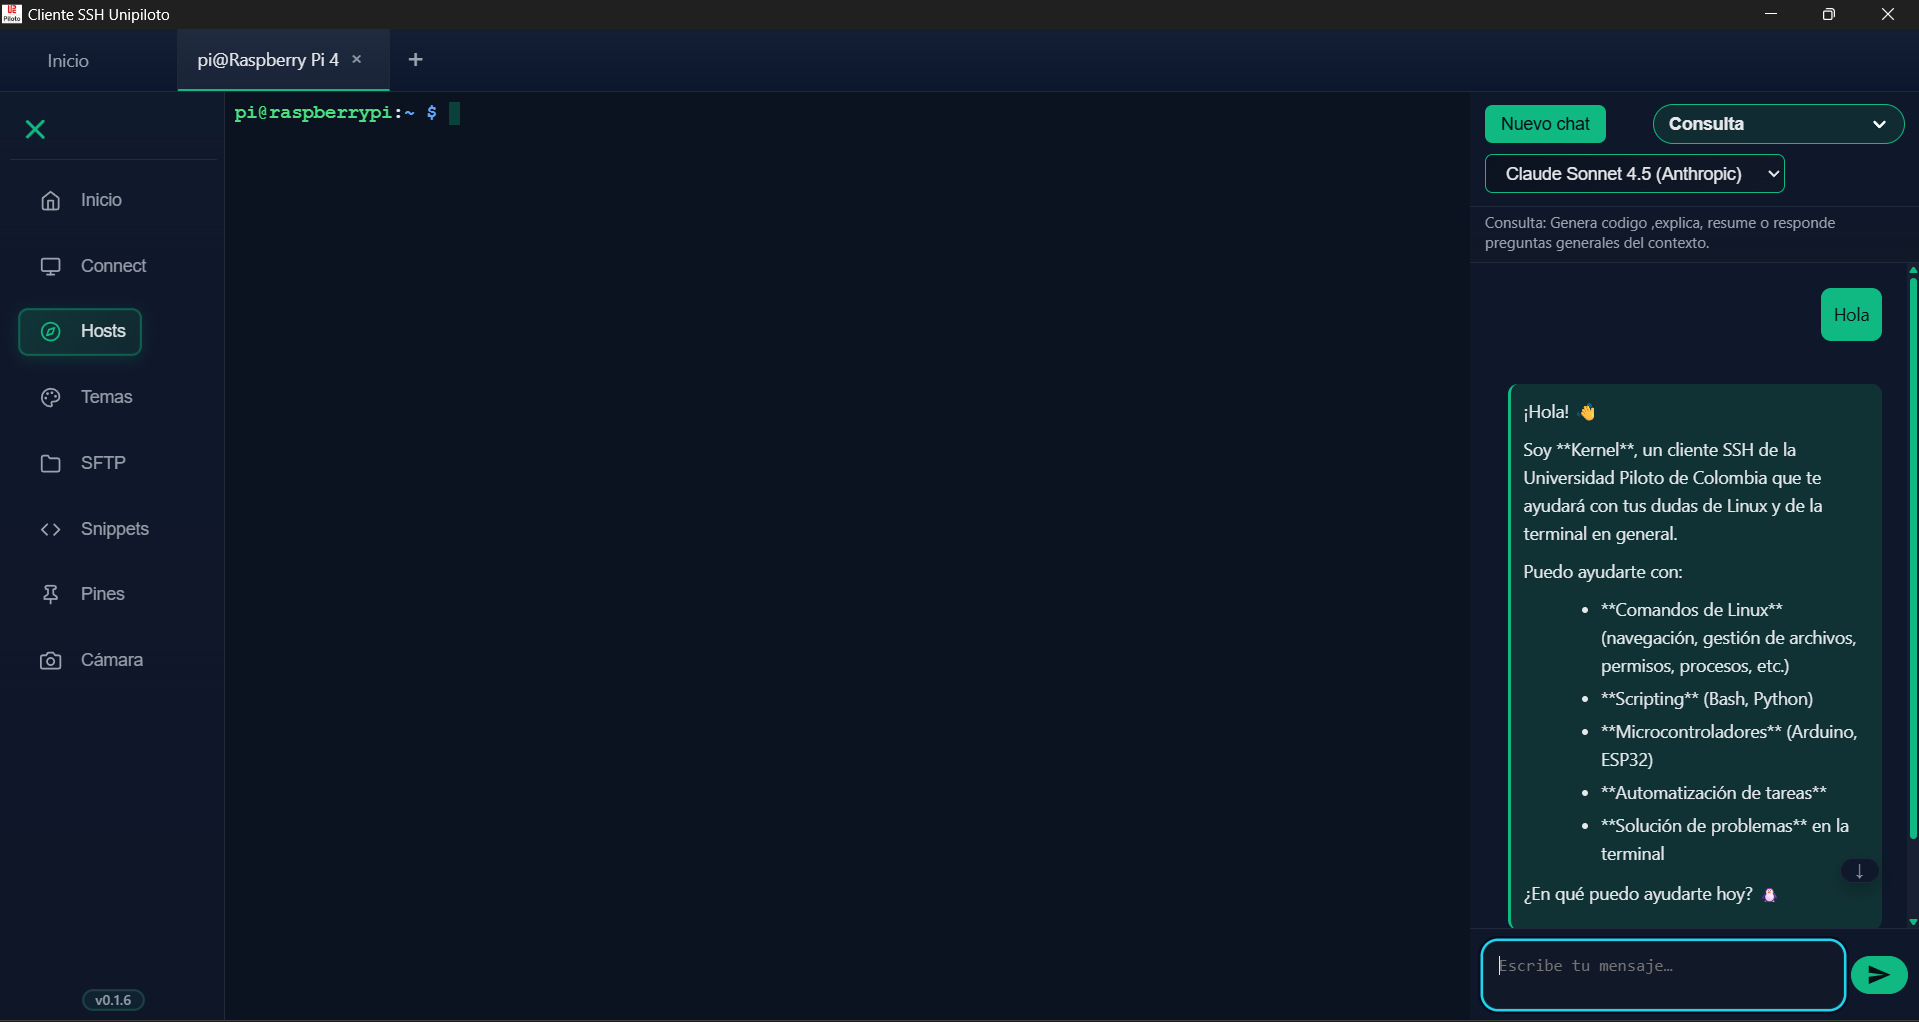
\includegraphics[width=\linewidth]{images/VistasoPrograma.png}
    \caption{Interfaz del programa en ejecución.}
    \label{fig:vistaso}
\end{figure}

\section{Trabajo Futuro}
Como líneas de trabajo futuro, se planea profundizar en la integración con modelos de IA, permitiendo al usuario elegir entre APIs comerciales (como ChatGPT de OpenAI o Gemini de Google) y soluciones de IA local (como Mistral) para garantizar la privacidad de los datos y evitar la sobrecarga del software con cálculos pesados en la nube.

Además, se propone añadir un botón de cambio rápido de idioma (español a inglés) directamente en la interfaz, facilitando su uso en entornos internacionales y bilingües.

\section*{Agradecimientos}
Se agradece a la Universidad, a los semilleros de investigación y a todos los integrantes del proyecto por el apoyo institucional y técnico brindado para la realización de este trabajo.

\section{Conclusiones}
El desarrollo de esta interfaz en Rust ha demostrado ser un éxito, proporcionando una herramienta robusta, segura y amigable para la administración de sistemas. El paper aporta una visión moderna de cómo la IA puede revitalizar el uso de la terminal.

Finalmente, las conclusiones se apoyan en la literatura existente que valida que "Linux y Rust van muy de la mano" \cite{ojeda2021rust}, destacando la creciente adopción de Rust dentro del propio kernel de Linux y su relevancia en el desarrollo de herramientas de sistema de próxima generación.

\bibliographystyle{IEEEtran}
\bibliography{bibliografia} % Llama al archivo bibliografia.bib
% -------------------

\end{document}